\documentclass[12pt]{article}
\usepackage{times}
\usepackage[english]{babel}
\usepackage[utf8x]{inputenc}
\usepackage[colorinlistoftodos]{todonotes}
\usepackage[margin=1in]{geometry}
\usepackage{graphicx}
\usepackage{epstopdf}
\usepackage{cite}
\usepackage{listings}
\usepackage{dtklogos}
\usepackage{wrapfig}
\usepackage{subfigure}
\usepackage{amsmath}
\usepackage{amsthm}
\usepackage{amssymb}
\usepackage{amscd}
\usepackage{caption}
\usepackage{etoolbox}
\usepackage{fancyhdr}
\usepackage{stackengine}
\usepackage[export]{adjustbox}
\usepackage{url}
\patchcmd{\thebibliography}{\section*{\refname}}{}{}{}
\usepackage[document]{ragged2e}    %This causes text to left align
\usepackage[colorlinks=true, linkcolor=black,citecolor=black,urlcolor=blue]{hyperref}
\bibliographystyle{IEEEtran}
\DeclareGraphicsRule{.tif}{png}{.png}{`convert #1 `dirname #1`/`basename #1 .tif`.png}

\title{MCHE 220: Report 1}

\begin{document}
\lefthyphenmin3
\righthyphenmin4
% \pretolerance=2000
% \tolerance=500 
% \emergencystretch=10pt
%\raggedright     %Stops LaTeX from automatically hyphenating the right margin to fit better
%Combine this with \usepackage[document]{ragged2e} to get a text align left similar to natural MS Word
%-------------------------------------------------------------
%Header
%-------------------------------------------------------------
\fancyhf{}  
  \renewcommand{\headrulewidth}{0pt}
  \fancypagestyle{plain}{
    \fancyhead[R]{\thepage}} 
    \pagestyle{plain}
    
\captionsetup[table]{labelsep=space}

\begin{flushleft}
\hrulefill\\\hrule height 1pt
\vspace{5pt}
\textbf{DATE: }\today
\bigskip\\
\textbf{TO: }Sally Anne McInerny, Ph.D.\\ Department of Mechanical Engineering
\bigskip\\
\textbf{FROM: }Matthew J. Begneaud
\bigskip\\
\textbf{COPY: }John Guillory, Ph.D.\\ Department of Mechanical Engineering
\bigskip\\
\textbf{SUBJECT:} Rubberband Stiffness Measurement
\vspace{-10pt}
\end{flushleft}
\hrulefill \hrule height 1pt

%-------------------------------------------------------------
%Start of Paper
%-------------------------------------------------------------

\section*{\fontsize{12}{12}\selectfont INTRODUCTION}
This memorandum is meant to convey the findings of an experiment conducted to observe the relation between force and deflection for rubber bands. The objectives of this experiment are to use force and elongation data to produce a regression model and to use this model to derive a relationship for the elastic energy stored in the rubber bands.
\bigskip

Because Hooke's Law only applies to small ranges of deflection where it is acceptable to assume a linear model, a more accurate model is desirable in order to expand the range in which the force-deflection relationship is known. The proposed model should look somewhat like a standard stress-strain curve, beginning with a steeper slope and then flattening out as the rubber band begins to deform past the elastic range \cite{rubberband_writeup}. This behavior refers to the typical true stress-true strain relation, which is a power law relation. It is expected that the data will follow the power law trend, and the regression model will be fitted to the data as such.


\section*{\fontsize{12}{12}\selectfont PROCEDURE}
The data collected from the test include forces recorded at various steps of the elongation. In the experiment, two rubber bands were connected to a hand-held fish weighing scale. The rubber bands were then stretched to various displacements and the resting force at each length was recorded. Four groups carried out the same procedure for eight different lengths and the data was combined to create a larger database.


\section*{\fontsize{12}{12}\selectfont DATA PRESENTATION \& ANALYSIS}
The raw data from the experiment can be seen in Figure 1. As predicted, the slope of the data seems to flatten out as the deflections increase in length. A power law regression has been fitted to the data, yielding a correlation coefficient of 0.9608. The Pr range for the regression is much less than 0.1\%. The resulting power law regression model can be seen in Equation (1). 
\bigskip

\begin{equation}
F = 0.5519x^{0.6253}
\end{equation}

% Data with power-law regression here
\begin{figure}[t!] %  figure placement: here, top, bottom, or page
   \centering
   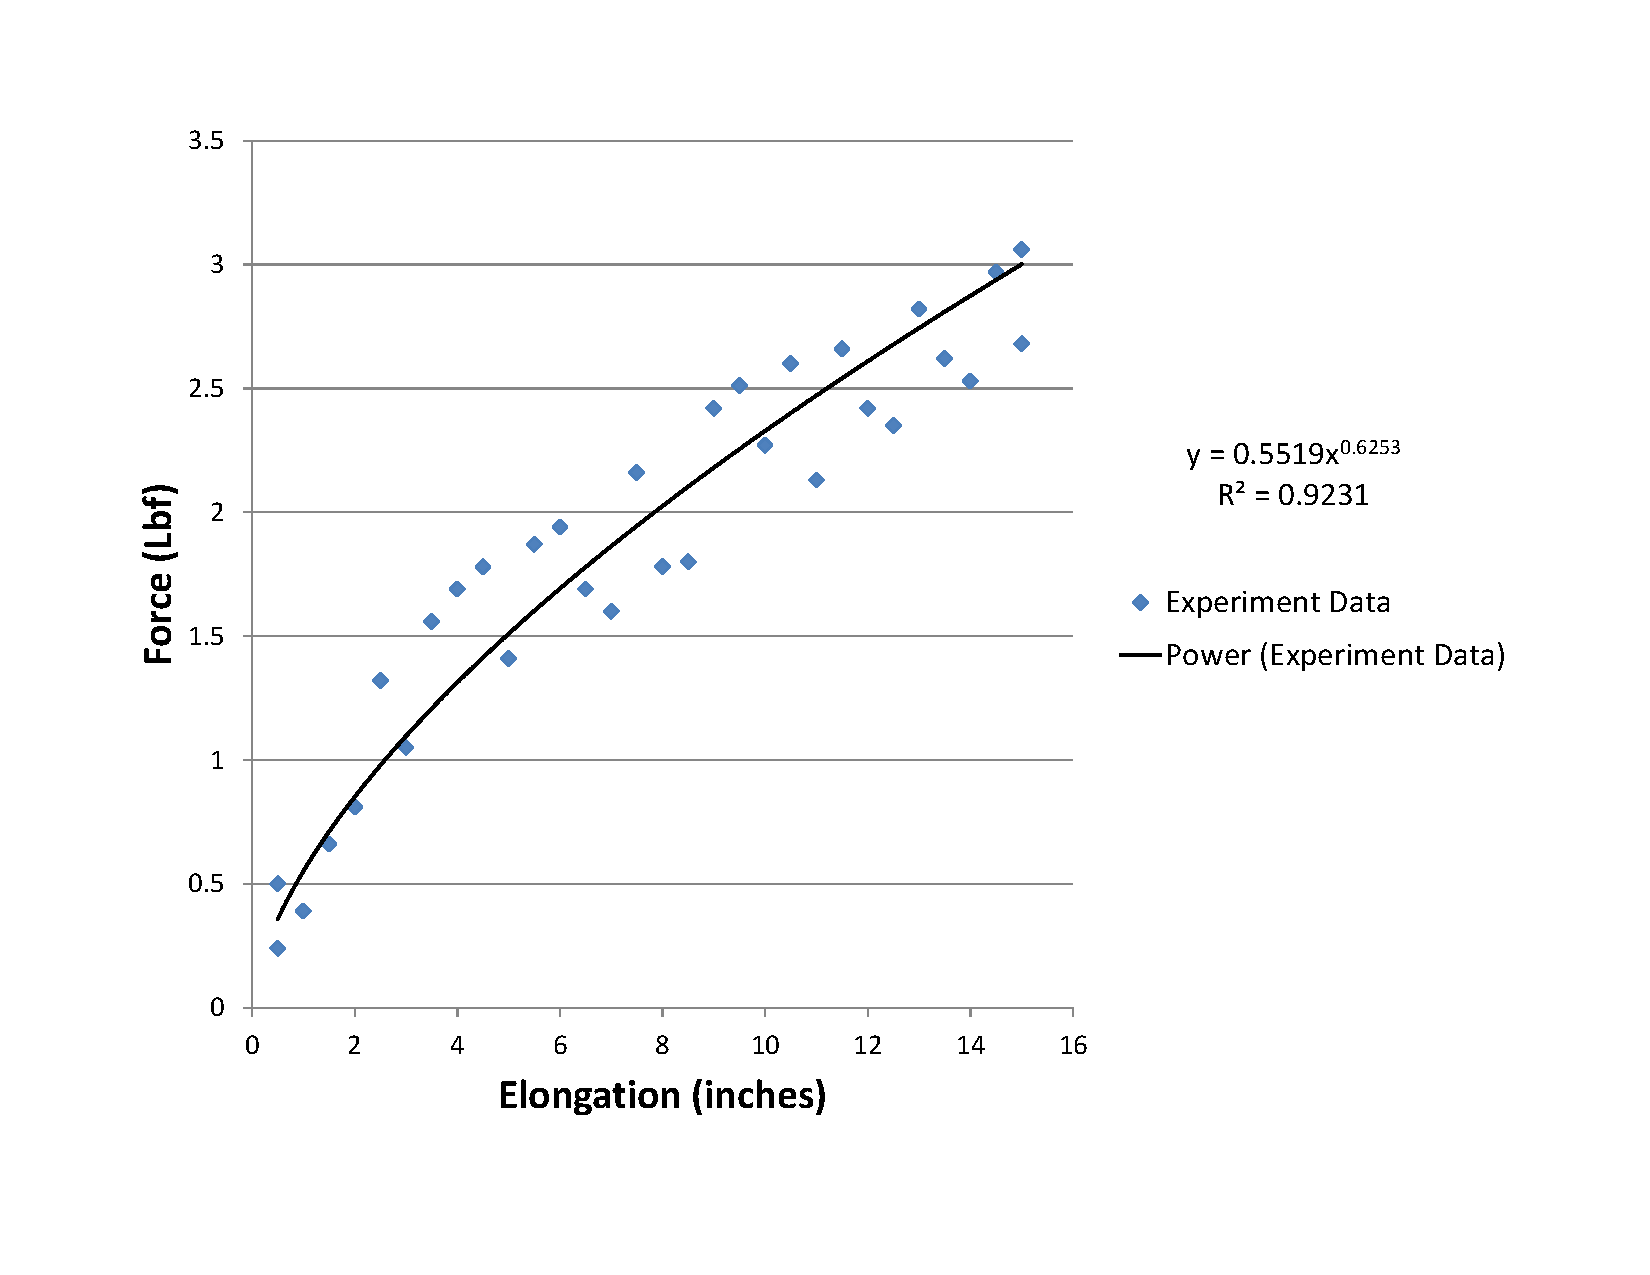
\includegraphics[width=\linewidth]{power_regression.pdf} 
   \caption{Experiment Data Fitted to Power-Law Regression Model}
   \label{fig:example}
\end{figure}

\bigskip
With a correlation coefficient of 0.9608, it is reasonable to attach a two-way range confidence of 95\%. At the mean value of deflections recorded, 7.75 inches, the confidence of estimate interval is found to be $1.986 \pm 0.015$ pounds. It is expected that due to the scattering of data as elongations get larger, that the range would increase as the deflection increases.
\bigskip

In order to derive a relationship for the elastic energy stored in the rubber bands, the regression model was integrated over the length of the displacements using the power rule, shown in Equation (2) and Equation (3). The representation of this relation can be seen in Figure 2.
\bigskip

\begin{equation}
E = \int_{0}^{\Delta L}Fdx
\end{equation}

\bigskip

\begin{equation}
E = \frac{0.5519x^{1.6253}}{1.6253}
\end{equation}

\newpage

% Energy relation graph here
\begin{figure}[t!] %  figure placement: here, top, bottom, or page
   \centering
   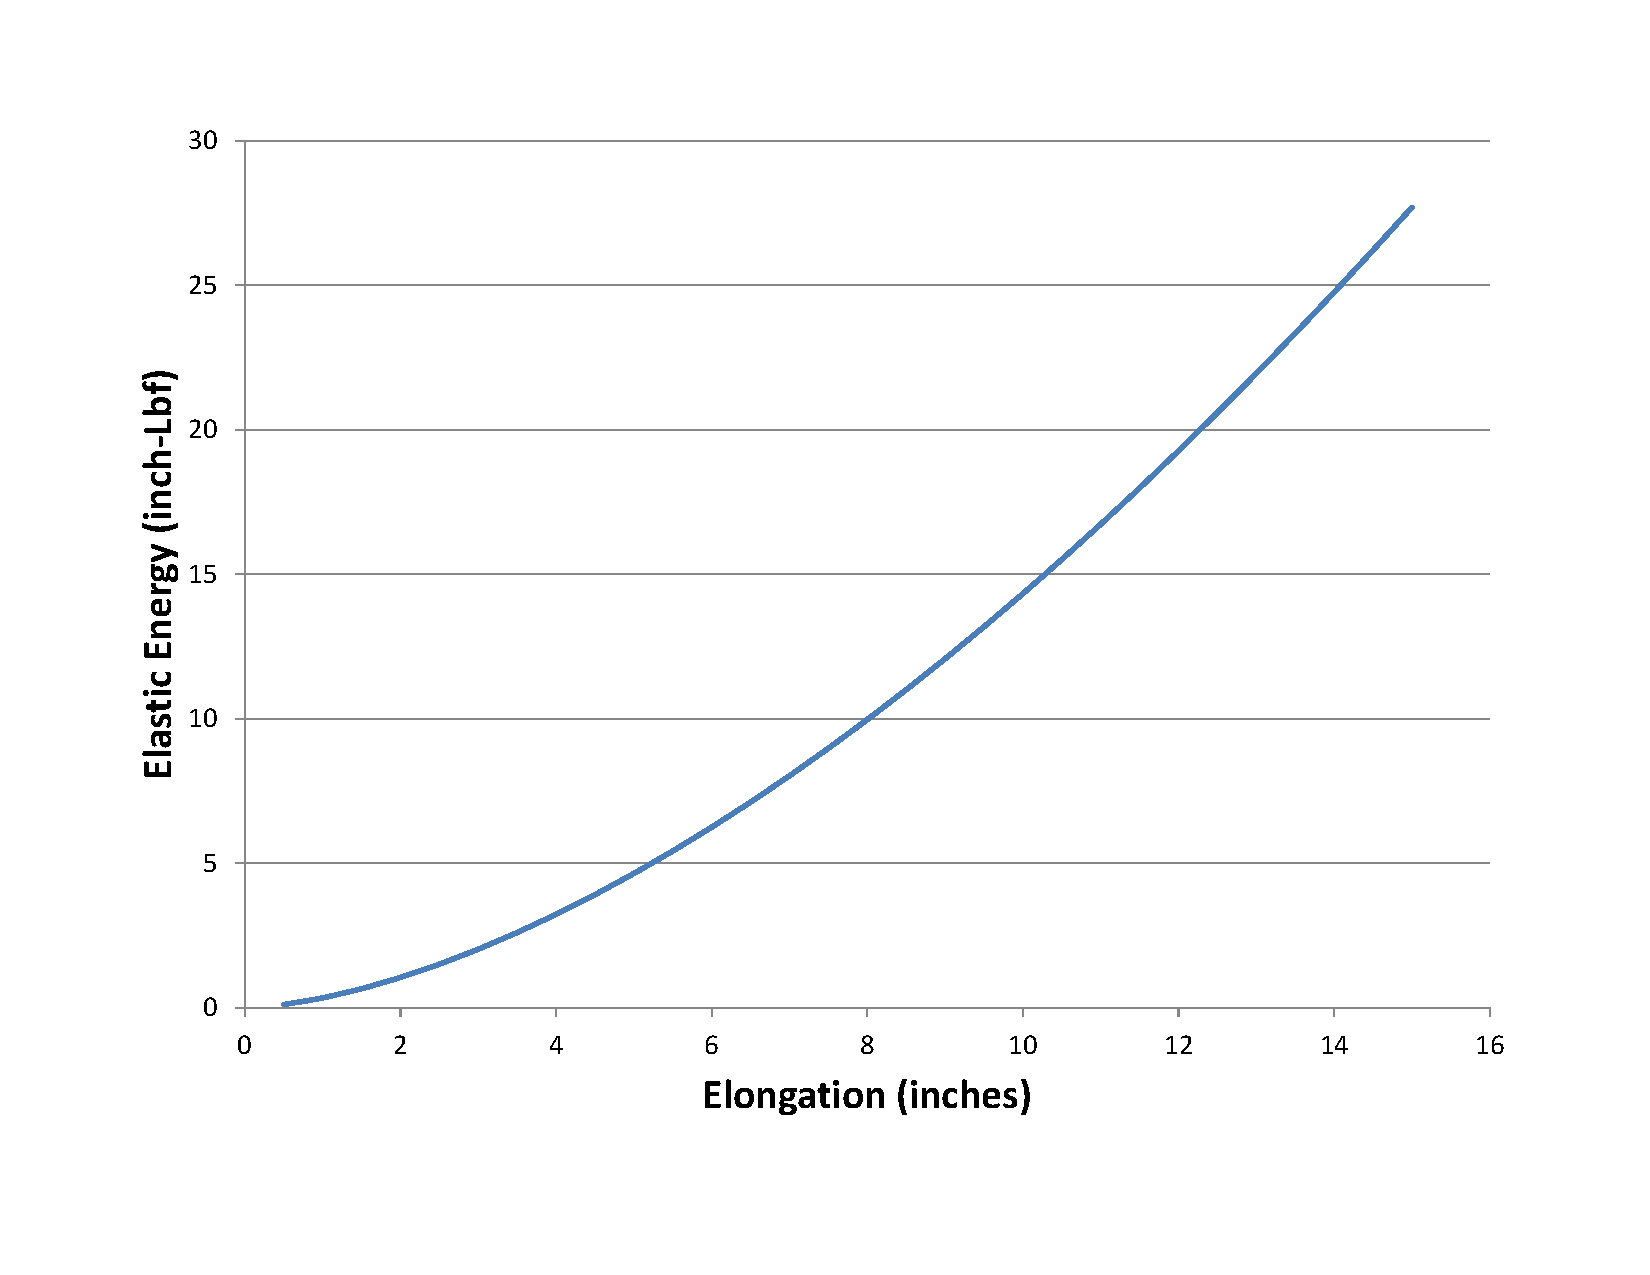
\includegraphics[width=\linewidth]{elastic_energy.pdf} 
   \caption{Experiment Data Fitted to Power-Law Regression Model}
   \label{fig:example}
\end{figure}

\bigskip



\section*{\fontsize{12}{12}\selectfont DISCUSSION}
As expected, the power-law regression model is a good fit for the data since the relation investigated by the experiment is essentially the true-stress true-strain relation, which itself is modeled by a power-law equation.
\bigskip

The data does seem to scatter much more in the upper-range of deflection values. It is likely due to the fact that as the rubber bands are stretched more, their imperfections and variances have a magnified effect on the stress imposed in the band. This means the regression model will lose accuracy as the rubber band is elongated further.


\section*{\fontsize{12}{12}\selectfont CONCLUSION}

\begin{itemize}
	\item The data from this experiment was fit to a power law regression model.
	\item The power law regression model fit the data quite well, yielding a correlation coefficient of $R=0.9608$ and a Pr range of much less than 0.1\%, proving that the model should be usable with high confidence of accuracy.
	\item At the mean value of deflections recorded, the confidence of estimate interval was found to be $1.986 \pm 0.015$.
	\item The regression model was used to derive a relation between the elastic energy stored in the rubber band and the displacement, or elongation, of the rubber band.
\end{itemize}

\bigskip


\section*{\fontsize{12}{12}\selectfont REFERENCES}

\begin{thebibliography}{2}

\bibitem{rubberband_writeup}
University of British Columbia, n.d., "Stretching Rubber Bands: Understanding Hooke's Law," from
\urlstyle{same}
 \url{http://c21.phas.ubc.ca/sites/default/files/rubber_band_write_up.pdf}

\end{thebibliography}

%\section*{\fontsize{12}{12}\selectfont APPENDIX}

%\begin{table}[h!]
%  \caption{}
%  \includegraphics[width=\linewidth]{table1.png}
%\end{table}

\end{document}
----------------------------%TEmplates-------------------------------

-------------------------Figure-----------------------

\begin{figure}[h!]  
  \centering
    \includegraphics[width=\linewidth]{**file**}
    \caption{Docking Station}
\end{figure}

---------------------------Table-----------------------
\begin{table}[ht]
\caption{Nonlinear Model Results} % title of Table
\centering % used for centering table
\begin{tabular}{c c c c} % centered columns (4 columns)
\hline\hline %inserts double horizontal lines
Case & Method\#1 & Method\#2 & Method\#3 \\ [0.5ex] % inserts table
%heading
\hline % inserts single horizontal line
1 & 50 & 837 & 970 \\ % inserting body of the table
2 & 47 & 877 & 230 \\
3 & 31 & 25 & 415 \\
4 & 35 & 144 & 2356 \\
5 & 45 & 300 & 556 \\ [1ex] % [1ex] adds vertical space
\hline %inserts single line
\end{tabular}
\label{table:nonlin} % is used to refer this table in the text
\end{table}



probably best to insert as an image from excel

\bigskip\\
\begin{table}[h!]
  \caption{}
  \includegraphics[width=\linewidth]{**file**}
\end{table}
\bigskip\\





-----------------------------Equations------------------------
-----------------------------Regular
\begin{equation}
a = b + c
\end{equation}

--------------------------------- Multiline
\begin{multline}
a = b + c + d + e + f
+ g + h + i + j \\
+ k + l + m + n + o
\end{multline}

-------------------------------Citations-------------------------
\bibitem{Author last name}
  Last, First., year of publication,
  article name, book(etc) name, from \\
  link goes here

----------------------------------other-----------------------------

equations:
http://moser-isi.ethz.ch/docs/typeset_equations.pdf

citations:
http://library.missouri.edu/engineering/about/guides/asme
https://www.asme.org/shop/proceedings/conference-publications/references